\chapter{Analysis}
\label{chap:analysis}
\section{Word Embedding: Word2Vec}
The main focus for this \gls{dp} is for the author to get some expertise with the Word Embedding [\ref{stoa:word-embedding}] and more specifically the Word2Vec [\ref{stoa:word2vec}, \ref{stoa:word2vec-pros-cons}] algorithm, which is already very complete on features and parameters\cite{article:word2vec-parameters}.



\subsection{Word2Vec Operations}
\subsubsection{Analogies}
\label{analyse:analogies}

Word2Vec is known for being able to handle analogies and more specifically for the famous:\\\\ \textit{Man is to Woman as King is to? \textbf{[Queen]}}\\ 

Which translated with Gensim [\ref{stoa:gensim}] into the vectorial form and the geometric operation as:
\begin{lstlisting}[language=Python]
model.wv.most_similar(positive=['king','woman'],
                    negative=['man'], topn=1)
\end{lstlisting}

Outputing the following: \textbf{[('queen', 0.6848626732826233)]}

\subsubsection{Geometric Operations}
\label{analyse:geometric-operations}
As each word in Word2Vec is a vector representation in a multi-dimensional space, it implies that standard geometrical operations are applicable. Indeed, as seen with analogies [\ref{analyse:analogies}], some operations are being made, implying \textit{positive} and \textit{negative}. Below are the top 3 operations used in the Word2Vec.

\begin{itemize}
    \setlength\itemsep{0em}
    \item Addition
    \item Soustraction
    \item Cosine
\end{itemize}

\subsubsection{Common Tasks}
\label{analyse:common-tasks}
As seen with analogies [\ref{analyse:analogies}], the \textit{most\_similar\(\)} function is a massively used task for Word2Vec, however it's not the only one. Indeed, the following is the top 3 functions used with Word2Vec space:

\begin{itemize}
    \setlength\itemsep{0em}
    \item most\_similar('king'): outputs the top most similar words to a given word.
    \item similarity('woman','man'): outputs the degree of similarity between two words.
    \item doesnt\_match('dog cat computer bird'.split\(\)): outputs the non similar words.
\end{itemize}


\subsection{Word Length}
\label{analyse:word-length}
As Word2Vec is a multi-dimension space, in which words are positioned, it is important to understand how those vectors are positioned and what information they carry. The word length represents how often a word is used in a context. Indeed, if a word is used a lot in a context, its length will be greater than the same word used at the same frequency but split up in multiple contexts. Meaning that word length, in combination with the term frequency, is useful to measure the word significance in contexts. \cite{article:word2vec-length}

\subsection{Word Angle}
\label{analyse:word-angle}
Word vectors are not only carrying the length [\ref{analyse:word-length}], they also have a direction, popularly described by the Cosine function. The process applied to vectors in Word Embedding is known as the Cosine Similarity, which is the vectors normalized dot product and making it very efficient for evaluation, in particular with sparse vectors such as word vectors.

\subsubsection{Positive Space}
Often, the Word2Vec space is kept into a positive space, implying that the output is between 0 and 1, where 1 is for the angle at 0\textdegree, which implies that vectors are above each other and the vectors are most probably the same.

\subsubsection{Negative Space}
However, it is also possible to go into the negative similarities, which is described by vectors being in opposite directions, with an angle higher than 90\textdegree, which transcribes into the -1 value if the vectors are in the exact opposites, independently to their magnitude. 


\subsection{Normalization}
\label{analyse:normalization}
During the similarity calculation, mathematically speaking normalizing vectors are making cosine [\ref{analyse:word-angle}] and dot-product equivalent. In word embedding, it is usually the relations between word vectors that are required, implying that to enhance the similarity function performances, the vector normalization is commonly used as in this case the length does not carry any useful information. However, if the relation to the context is required, the normalization should be avoided. 


\subsection{Lemmatization}
\label{analyse:lemmatization}
Expect from its direct implication with the dictionary size and its implication related to the processing power\/time required to compute the model. Lemmatization should be considered in specific cases. Indeed, using it makes the Word2Vec space sparser, which is useful for small datasets; however, for big datasets, the gain is often negligible. \\

However, for the case where the words must carry different information depending on the context, for instance with abbreviations, it is necessary to use the lemmatization feature, for example, \gls{ir} could be mistaken with Infrared (IR).\\

Another case would be the need for the use of tokens for written words such as \textit{New York}.


\subsection{\gls{cbow}}
\label{analyse:cbow}
Continues Bag of Words is the original method presented in the Word2Vec paper \cite{article:word2vec}  and involves \gls{nn} to predict a word vector based on its context. In the case of a unique word vector, it is similar to an encoder-decoder architecture.\\

The concept behind \gls{cbow} is to take, for a given word vector, the \textit{n} neighboring word vectors as the context, then predict the given word vector, as seen on the figure \ref{fig:wikipedia_cbow_skipgram_img}.\\

Concerning the prediction quality, its measure requires to provide the hot encoding of the given word as input, so it calculates the output error and learns the vector representation of the word.

\subsection{Skip-Grams}
\label{analyse:skip-grams}
Introduced by facebook, Fasttext\cite{article:fasttext} Word Embedding is using a variant of \gls{cbow} that looks like its flipped version, as seen on figure \ref{fig:wikipedia_cbow_skipgram_img}. It also involves a \gls{nn}, but instead of predicting the word based on the context, it predicts the context based on the word.\\

Given the target word vector as input, the model outputs the probability distribution for the given word.

\begin{figure}[ht!]
    \centering
    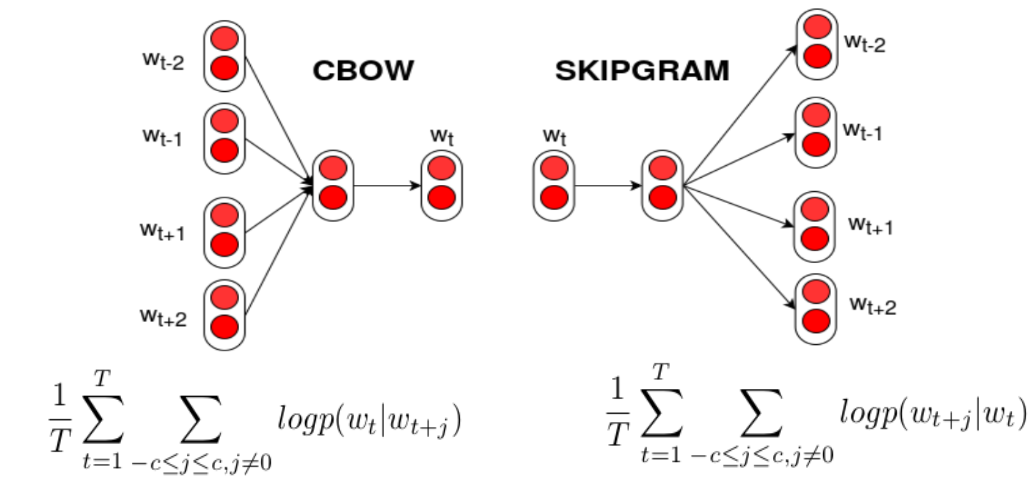
\includegraphics[width=\textwidth,height=6cm,keepaspectratio=true]{CBOW_eta_Skipgram}
    \caption{
       CBOW and Skip-Gram neural network representations\cite{wikipedia:cbow_skipgram_img}
    }
    \label{fig:wikipedia_cbow_skipgram_img}
\end{figure}

\subsection{Dimensions}
\label{analyse:dimensions}
Typically between 100 and 400, Word2Vec dimensions are defining the accuracy in the similarity between word vectors. It is difficult to find the sweet spot. However, there is some experimental curve for the dimension amount, which takes into account the final accuracy, time, and power consumption. 

\paragraph{Low accuracy}
It is recommended to use at least 50 dimensions to avoid loosing too many properties of high dimensions.

\paragraph{Normal accuracy}
Using around 200 dimensions provides acceptable accuracy for the time spent computing.

\paragraph{High accuracy}
Around 300 dimensions, the results are considered very good; however, the time is high.

\paragraph{Beyond high accuracy}
It seems that beyond 300 dimensions the accuracy gain is not worth anymore the extra time used during training.\\

In other words, the amount of dimensions usually reflects the over and underfitting of the model. Each model is dependent on the dataset, and it is often required to test the different number until the accuracy is acceptable. Plus, as this subject is still debated at the moment in the \gls{ml} community, there is no absolute value, except try and fail.


\subsection{Window}
\label{analyse:window}
As explained for \gls{cbow}\ref{analyse:cbow} and Skip-Grams\ref{analyse:skip-grams}, those algorithms are either taking the context as input, or outputting the context for a given word. However, to capture the context, it is required to define its size, which is in our case called the window.\\

By default, the value of  5 of the window is used and generally works well; however, the accuracy of the model will depend on the dataset used.\\

As a measure, the analogy score could be used. However, this score is often not the solution as the impact of the quality of a poor dataset is higher than the size of the window if using the default value. Plus it is essential to be careful with the sentence sizes of the corpus used; indeed, if the window value is higher to the average sentences length, the algorithm will not capture meaningful relations. \\

In other words, large windows size usually capture more information related to the main topic, and small windows are capturing the information related to the word itself.


\subsection{Epochs}
\label{analyse:epochs}
As the number of epochs is directly proportional to the amount of computation and time spent training the model, the common question to ask is: \textit{How much epochs will be giving the best accuracy for the time spent?} The answer is as always: it depends on the dataset and the parameters. \\

However, based on various sources, including the author of Gensim\cite{article:word2vec-epochs}, it is suggested that increasing the number of epochs have, in most of the case, an accuracy performance. The default value is usually five epochs.\\

Finally, the quest to find the right parameters is still a matter of experimentations.


\subsection{Gensim API}
It would not make much sense to go in details of each Gensim parameter, as a list of the parameters, and their description is available on their official API website\cite{article:gensim-api}.

However, to initiate the curiosity of the reader, the following list represents the most used parameters during the \gls{dp}:

\begin{itemize}
    \setlength\itemsep{0em}
    \item size: dimensions used [\ref{analyse:dimensions}]
    \item window: window size used [\ref{analyse:window}]
    \item min\_count: minimum frequency a word should have to be considered
    \item workers: cpu cores used
    \item sg: set at 1 to use Skip-Grams [\ref{analyse:skip-grams}] and set at 0 to use \gls{cbow} [\ref{analyse:cbow}]
    \item iter: epochs used [\ref{analyse:epochs}]
\end{itemize}


\subsection{Retrain Model}
\label{analyse:retrain}
In \gls{ml}, models are the resulting artifacts from training processes and provide the rules to generate an output for an input. A Word2Vec model is the representation of the relations between the dictionary of words and their contexts for the corpus it was trained on.\\

As seen in the state of the art section, pre-trained Word2Vec models are available on the internet [\ref{sota:word2vec-models}]. However, to save disk space and probably business knowledge, it is infrequent that the full model is shared. Indeed, the model provided an only a model with frozen \gls{ann} weights, which is perfectly fine for regular usage as it behaves the same as a full model, except that it is not containing the multi-dimensional matrix representing the Word2Vec space.\\

To get the full model, it requires to train it ourselves, with all the side-effects it implies, such as having a high amount of power and time consumption. However, a full model provides the ability to \textit{retrain} the model. One could add words to the dictionary or customize the weights to match a new verbal style or context. For instance, starting from on a Wikipedia model, it would be possible to influence the words to match the style of an author such as \textit{Edgar Allan Poe}.


\subsection{Evaluation}
\label{analyse:evaluation}
Determining if the model makes works correctly is difficult, a naive solution would be to create a complex supervised protocol to evaluate the success of a model. However, it would not require an enormous amount of work from a human perceptive. A solution is to exploit the analogies capabilities from Word2Vec \ref{analyse:analogies}, which, in theory, should perform well at.\\

The concept is called the \textit{Analogy Evaluation} and it uses a list of pre-made analogies in various domaines, such as the famous: \textbf{Man is to King, as Woman is to?}, and evaluate if the results from the model match the expect answer: \textit{Queen}. In Gensim, the following function does the evaluation: 
%[language=Python]
\begin{lstlisting}
evaluate_word_analogies(analogies,
                        restrict_vocab=300000,
                        case_insensitive=True,
                        dummy4unknown=False)
\end{lstlisting}
\vspace{1em}

Another evaluation method would be based on the word similarities itself. Indeed, based on a pre-made list of pairs of words, an input such as \textit{cup} would output \textit{mug}. This evaluation is done in Gensim via the following function:

%[language=Python]
\begin{lstlisting}
evaluate_word_pairs(pairs, delimiter='\t',
                    restrict_vocab=300000,
                    case_insensitive=True,
                    dummy4unknown=False)
\end{lstlisting}


\subsection{CPU VS GPU}
As mentioned in the state of the art section, Word2Vec is performing better than \gls{dl} solutions, in the most cases, because it is not using labeled data [\ref{sota:rnn}], even with the use of GPUs. However, in the context of Word2Vec, an experiment from Gensim has been made to compare the computation made CPU and GPU on the Gensim Framework \cite{article:word2vec-cpu-gpu}. The result is unexpected from a generalization point of view: indeed, it appears that CPUs are performing better than GPUs during the Word2Vec training.

